\documentclass[12pt, a4paper]{article}
\usepackage[english]{babel}             % Inglés para los nombres
\usepackage[utf8]{inputenc}             % Codificación de entrada
\usepackage[T1]{fontenc}                % Codificación de fuente (escribir castellano)
\usepackage{lmodern}                    % Fuente (la default no es compatible con castellano)
\usepackage{csquotes}                   % Para comillas y otras anotaciones del castellano
\usepackage{fancyhdr}                   % Encabezado y Pie de pagina
\usepackage{tocloft}                    % Puntos en los índices

\usepackage{url}                        % 
\usepackage{hyperref}                   % Links y referencias dentro del texto
\usepackage{nameref}                    % Para poder referenciar por nombre
\usepackage{acronym}                    % Para incluir las listas de abreviaturas
\usepackage{multicol}                   % Permite crear espacios con columnas verticales
\usepackage{booktabs} % Para mejores líneas horizontales en tablas
\usepackage{parskip}                    % Eliminar sangrado y añadir espacio entre párrafos
\usepackage{titlesec}                   % Crear subsubsub secciones
\usepackage{amsmath}                    % Funciones para ecuaciones
\usepackage{blkarray}                   % Matrices con anotaciones
\usepackage{algorithm}                  % Algoritmos con formalismos
\usepackage{algpseudocode}              % También para algoritmos
\usepackage{listings}                   % Para insertar codigo

\usepackage{array}                      % Para personalizar columnas de tabla
\usepackage{tabularx}                   % Para tablas de ancho variable

\usepackage{graphicx}                   % Para incluir imágenes
\usepackage{subcaption}                 % Subfiguras
\usepackage[table]{xcolor}              % Definir y utilizar colores
\usepackage{tikz}                       % Dibujar formas, figuras, rectas, intersecciones...
\usepackage[absolute,overlay]{textpos}  % Posición absoluta para textos
\usepackage{geometry}                   % Para controlar los márgenes

\usepackage{float}
\usepackage{soul}                       % Para highligths \hl
\usepackage{lipsum} 

\usepackage[backend=biber, sorting=none]{biblatex} % Referencias (bibliografía / webgrafía)
\selectlanguage{english}                % Seleccionar inglés
\bibliography{referencias}              % Incluir el archivo de referencias

\setlength{\emergencystretch}{3em}

% Definición de nombres
%\printbibliography[title={Bibliografía}]
\renewcommand{\cftsecleader}{\cftdotfill{\cftdotsep}} 
\newcommand{\student}{García Justel, Alan}
\newcommand{\director}{ Barrena Orueechebarria, Nagore; Elordi Hidalgo, Unai}
\newcommand{\codirector}{Sánchez Juanola, Martí}
\newcommand{\master}{ COMPUTATIONAL ENGINEERING AND INTELLIGENT SYSTEMS}
\newcommand{\titulo}{VEHICLE SCENES PREANOTATION WITH MONOCULAR SEMANTIC SEGMENTATION}
\newcommand{\portada}{images/shared/no_signal.jpg}
\newcommand{\curso}{2024-2025}

% Definición de Macros
\newcommand*{\fullref}[1]{\hyperref[{#1}]{\autoref*{#1} \nameref*{#1}}} % One single link

\newcommand{\aclink}[1]{% Crear links a acronimos
  \ifcsdef{ac@#1}{%
    \ifcsdef{mark@#1}{%
      \hyperlink{acro:#1}{\acs{#1}}%
    }{%
      \hyperlink{acro:#1}{\ac{#1}}%
      \expandafter\gdef\csname mark@#1\endcsname{}%
    }%
  }{%
    \ac{#1}%
    \expandafter\gdef\csname mark@#1\endcsname{}%
  }%
}

% Notas en Figuras
\newcommand\fnote[1]{\captionsetup{width=0.8\linewidth, font=footnotesize}\caption*{#1}}

% Estilos de listings
% Configuración del estilo para resaltar el código de ROS
\lstdefinestyle{ros}{
    backgroundcolor=\color{white}, % Cambiar el color de fondo
    basicstyle=\small\ttfamily, % Texto más pequeño
    breaklines=true,
    language=C,
    morekeywords={int32, float64},
    keywordstyle=\color{blue},
    commentstyle=\color{green!40!black},
    stringstyle=\color{red},
    breakatwhitespace=false,         
    breaklines=true,                 
    captionpos=b,                    
    keepspaces=true,                 
    numbers=left,                    
    numbersep=5pt,                  
    showspaces=false,                
    showstringspaces=false,
    showtabs=false,                  
    tabsize=2
}

% Crear subsubsub secciones
\titleclass{\subsubsubsection}{straight}[\subsection]
\newcounter{subsubsubsection}[subsubsection]
\renewcommand\thesubsubsubsection{\thesubsubsection.\arabic{subsubsubsection}}
\renewcommand\theparagraph{\thesubsubsubsection.\arabic{paragraph}} % optional; useful if paragraphs are to be numbered

\titleformat{\subsubsubsection}
  {\normalfont\normalsize\bfseries}{\thesubsubsubsection}{1em}{}
\titlespacing*{\subsubsubsection}
{0pt}{3.25ex plus 1ex minus .2ex}{1.5ex plus .2ex}
\makeatletter
\renewcommand\paragraph{\@startsection{paragraph}{5}{\z@}%
  {3.25ex \@plus1ex \@minus.2ex}%
  {-1em}%
  {\normalfont\normalsize\bfseries}}
\renewcommand\subparagraph{\@startsection{subparagraph}{6}{\parindent}%
  {3.25ex \@plus1ex \@minus .2ex}%
  {-1em}%
  {\normalfont\normalsize\bfseries}}
\def\toclevel@subsubsubsection{4}
\def\toclevel@paragraph{5}
\def\toclevel@paragraph{6}
\def\l@subsubsubsection{\@dottedtocline{4}{7em}{4em}}
\def\l@paragraph{\@dottedtocline{5}{10em}{5em}}
\def\l@subparagraph{\@dottedtocline{6}{14em}{6em}}
\makeatother
\setcounter{secnumdepth}{4}
\setcounter{tocdepth}{4}



% Encabezado y Pie de pagina
\pagestyle{fancy}                       % Estilo de las páginas
\fancyhf{}
\fancyhead[L]{Master's Thesis}
\fancyhead[R]{\leftmark}
\fancyfoot[L]{UPV/EHU}
\fancyfoot[R]{\thepage}
\renewcommand{\footrulewidth}{0.4pt} % Línea horizontal en el pie de página
\setlength{\headheight}{15.5pt}

% Definición de colores
\definecolor{ehu_blue}{HTML}{376092}
\definecolor{link_color}{HTML}{36AEB4}
\definecolor{reference_color}{HTML}{0F3133}
\definecolor{cite_color}{HTML}{ff7f42}
\definecolor{table_gray}{HTML}{C0C0C0}
\definecolor{table_red}{HTML}{fb4952}


% Incluye todas las entradas del archivo .bib en la bibliografía
\nocite{*}

% Configuración de hyperref para diferentes tipos de enlaces
\hypersetup{
    colorlinks=true,
    linkcolor=reference_color,
    citecolor=cite_color,
    filecolor=link_color,
    urlcolor=link_color,
}

% #########################################################################
% #                                  TFM                                  #
% #########################################################################
\begin{document}
\newgeometry{bottom=2cm}

\begin{titlepage}
    % Logo de la universidad
    \begin{textblock*}{\textwidth}(10cm,0cm)
        
\includegraphics[width=7.5cm, height=3cm]{images/shared/Logo_EHU.jpg}
    \end{textblock*}
    
    % Franja azul
    \begin{tikzpicture}[remember picture, overlay]
        \fill[ehu_blue] (current page.north west) ++ (0,-3.01cm) rectangle (\paperwidth,-3cm);
    \end{tikzpicture}
    
    \begin{textblock*}{\paperwidth}(\dimexpr\parindent+\oddsidemargin+3em\relax,3.5cm)
        \begin{minipage}{\dimexpr\linewidth-7.5cm\relax}
            \color{white}
            \noindent\rule{\linewidth}{0cm}
            \textsf{ {\large MÁSTER EN \master}}
            \newline
            \newline \newline
            \textsf{\textbf{ {\Huge TRABAJO FIN DE MÁSTER }}}
        \end{minipage}
    \end{textblock*}
    
    % Título del trabajo
    \vspace*{3.5cm}
    \begin{minipage}{\linewidth}
        \setlength{\baselineskip}{1.7\baselineskip}
        \centering
        \textsf{ \textbf{ {\LARGE \titulo }}}
    \end{minipage}

    % Foto de portada
    \vspace*{0.5cm}
    \begin{figure}[H]
        \centering
        \includegraphics[width=10cm, height=8cm]{\portada}
    \end{figure}

    % ODS
    \vspace*{1cm}
    % \begin{figure}[h]
    % \centering
    %     \begin{subfigure}[b]{0.135\textwidth}
    %         \includegraphics[width=2cm, height=2cm]{images/iconos_ods/03.png}
    %     \end{subfigure}
    %     \begin{subfigure}[b]{0.135\textwidth}
    %         \includegraphics[width=2cm, height=2cm]{images/iconos_ods/04.png}
    %     \end{subfigure}
    %     \begin{subfigure}[b]{0.135\textwidth}
    %         \includegraphics[width=2cm, height=2cm]{images/iconos_ods/05.png}
    %     \end{subfigure}
    %     \begin{subfigure}[b]{0.135\textwidth}
    %         \includegraphics[width=2cm, height=2cm]{images/iconos_ods/07.png}
    %     \end{subfigure}
    %     \begin{subfigure}[b]{0.135\textwidth}
    %         \includegraphics[width=2cm, height=2cm]{images/iconos_ods/08.png}
    %     \end{subfigure}
    %     \begin{subfigure}[b]{0.135\textwidth}
    %         \includegraphics[width=2cm, height=2cm]{images/iconos_ods/09.png}
    %     \end{subfigure}
    %     \begin{subfigure}[b]{0.135\textwidth}
    %         \includegraphics[width=2cm, height=2cm]{images/iconos_ods/12.png}
    %     \end{subfigure}
    % 
    %     \label{fig:ods-iconos}
    % \end{figure}
    
    % Estudiante
    \vspace{0.2cm}
    \noindent {\footnotesize \textbf{Estudiante:} \estudiante}
    \newline
    \noindent\makebox[\linewidth]{\rule{\textwidth}{0.4pt}} % Línea horizontal

    % Director
    \nopagebreak
    \vspace{0.3cm}
    \nopagebreak
    \noindent {\footnotesize \textbf{Director/Directora:} \director }

    % Espacio para firmas
    \vspace{0.5cm} % Espacio entre texto "Director/Directora" y espacio para firmas
    \noindent 
    \makebox[0.4\linewidth]{\hrulefill}
    \hspace{0.2\linewidth}
    \makebox[0.4\linewidth]{\hrulefill}

    % Curso y Fecha
    \vspace{0.1cm}    
    \noindent {\footnotesize \textbf{Curso: } \curso \hfill \textbf{Fecha:} \today }
\end{titlepage}

\restoregeometry
\setcounter{figure}{0} % Incluimos el título

% \newpage % BORRAR EN LA VERSIÓN FINAL
% \input{notas}

\newpage
\markboth{Summary}{Summary}
\begin{itshape}
    \textbf{Resumen:} \\
    
    \textbf{Palabras Clave: }
\end{itshape}
\newpage

\begin{itshape}
    \textbf{Abstract:} \\

    \textbf{Key Words: }
\end{itshape}
\newpage

\begin{itshape}
    \textbf{Laburpena:} \\

    \textbf{Gako-hitzak: }
\end{itshape}

\newpage

 % Incluimos el resumen tri-lingüe

% Índices
\tableofcontents\thispagestyle{empty}\newpage
\listoffigures\thispagestyle{empty}\newpage
\listoftables\thispagestyle{empty}\newpage

% Abreviaturas
\section*{Abbreviations}
\markboth{Abbreviations}{Abbreviations}
\addcontentsline{toc}{section}{Abbreviations}
%\begin{multicols}{2} % Si se quieren en dos columnas verticales
\begin{acronym}[ADAS]  % El acrónimo más largo
    \acro{TFM}{Trabajo Fin de Máster}
    \acro{ADS}{Automated Driving Systems}
    \acro{ADAS}{Advanced Driving Assistance Systems}
    \acro{SAE}{Society of Automotive Engineers}
    \acro{V2I}{Vehicle-to-Infrastructure}
    \acro{V2X}{Vehicle-to-Everything}
    \acro{BEV}{bird's-eye-view}
    \acro{LiDAR}{Light Detection and Ranging}
    \acro{IPM}{Inverse Perspective Mapping}
\end{acronym}
%\end{multicols}

 % Marcar como visto (No te desglosa el acrónimo)
 % Provoca warnings pero funciona :)
\acused{ADAS}
\acused{LiDAR}
\newpage

\section{Introduction}
\label{Introduction}
% ================================================
% =                INTRODUCTION                  =
% ================================================ 

The development of \aclink{ADS} has been a hot topic in the automotive industry for the last years. One of the fundamental aspects of an \aclink{ADS} is its perception system, as it is responsible for performing the obstacle detection and to provide a good environment representation for other systems, among others. This perception system can be divided into two main tasks: 3D object detection and local \aclink{BEV} map generation. 

3D object detection is usually based on pointclouds obtained from \aclink{LiDAR} sensors, but as this sensors are costly a lot of research has been made in the field of camera 3D object detection. This approach has been gaining a lot of popularity carried by the improvemnts of the computer vision techniques with deep learning.

\aclink{BEV} segmentation aims to create a semantic representation of a vehicle's surroundings. This is a key component of an \aclink{ADS} perception system as \aclink{BEV} segmentation provides rich semantic information, precise localization, and absolute scales. This makes it useful for various tasks, including map reconstruction, prediction of agent intentions, and vehicle path planning.

To obtain \aclink{BEV} semantic segmentation from cameras, traditional methods first generate semantic masks in image space and then transform them into \aclink{BEV} space using \aclink{IPM}. Although simple, it requires accurate camera parameters and assumes a perfectly flat ground surface, which limits its effectiveness. Moreover, while planar or low-height objects such as road curbs, lane markings, and the drivable area retain a meaningful metric representation in \aclink{BEV} space, objects with height appear distorted after the transformation.

With the objective of addressing this limitations, recent methods leverage data-driven techniques for \aclink{BEV} representation. \cite{view_parsing_network} \cite{lift_splat_shoot} \cite{m2bev}. However, to the best of our knowledge, no previous work has explored training a standard semantic segmentation model directly on \aclink{BEV} images to measure the difference between the inference of planar elements.

This master's thesis seeks to answer the question: \textit{Does a model directly trained on semantic BEV images outperforms a typical segmentation model for plannar elements?}. Additionally, this work explores a technical application of \aclink{BEV} semantic segmentation for annotating vehicular scenes with occupancy, occlusion, and drivable area masks, contributing to the field of monocular 3D object detection given 2D semantic masks.



\section{State of the art}
\label{sota}
% ================================================
% =              STATE OF THE ART                =
% ================================================ 
Actualmente, la industria de la automoción está impulsando el desarrollo de los \aclink{ADS} con la promesa de reducir los accidentes en carretera y minimizar los costes tanto humanos como económicos que estos suponen \cite{survey_AutomatedDriving1}. Sin embargo, a pesar de que la conducción automatizada haya incrementado recientemente la atención de la industria por el auge del DeepLearning y la visión por ordenador, lo cierto es que lleva presente más de 20 años.

Algunas de las primeras competiciones de conducción automatizada, como los DARPA Challenges en 2003 y 2005 o el Grand DARPA Urban challenge de 2007, impulsaron enormemente el desarrollo de los \aclink{ADS}, atrayendo la atención tanto de empresas tecnológicas como del sector automotriz \cite{survey_AutomatedDriving2}. Este avance ha sido acompañado por la definición de buenas prácticas y procesos de estandarización para garantizar la seguridad y fiabilidad de los \aclink{ADS}. En este contexto, la \aclink{SAE} ha establecido una escala progresiva de automatización, desde el nivel 0 (sin automatización) hasta el nivel 5 (automatización total), definiendo el grado de intervención del conductor en cada etapa \cite{AD_Technical_Standards}. 

Hoy en día, la mayoría de los vehículos incorporan sistemas avanzados de asistencia a la conducción \aclink{ADAS}, que operan en los niveles \aclink{SAE} 2 y 3. No obstante, ya existen \aclink{ADS} de nivel 4, como los desarrollados por Waymo y Cruise para robotaxis, o los autobuses autónomos desplegados en algunas ciudades, cuyos sistemas están diseñados para gestionar el fallback de manera autónoma, sin necesidad de intervención humana \cite{fallback_strategy}.

Este desarrollo ha llevado a la creación de distintas estrategias y arquitecturas para los \aclink{ADS}. En los últimos años, ha habido grandes avances en soluciones \mbox{End-to-End}, que combinan técnicas de aprendizaje profundo y aprendizaje por refuerzo para obtener las acciones de control del vehículo partiendo diréctamente de los datos de los sensores \cite{end_to_end_driving}. Sin embargo, la mayoría de los enfoques optan por soluciones modulares más tradicionales, que dividen el problema de la conducción automatizada en \mbox{sub-tareas} específicas, integrando soluciones de campos como la robótica, visión por ordenador, deep learning y control automático.

En el contexto de las arquitecturas modulares, la adopción de buenas prácticas ha facilitado la categorización de estas \mbox{sub-tareas} en tres grupos principales \cite{machines5010006}\cite{functional_architectures}: 
\begin{itemize}
    \item Percepción, que se refiere a la capacidad del sistema autónomo para recolectar información del entorno y extraer conocimiento relevante, como la ubicación de obstáculos, señales de tráfico y la localización del vehículo.
    \item Planificación del comportamiento, que consiste en tomar decisiones para alcanzar los objetivos del vehículo, como llegar de un punto a otro evitando obstáculos y optimizando la trayectoria.
    \item Ejecución de movimientos, que se refiere a la capacidad del vehículo para ejecutar las acciones planificadas por el sistema, controlando la dirección, velocidad y maniobras necesarias.
\end{itemize}
Además, estas \mbox{sub-tareas} interactúan entre sí, con el hardware del vehículo y con sistemas de comunicación como \aclink{V2I} o \aclink{V2X} en el caso de los vehículos conectados.

\begin{figure}[H]
    \centering
    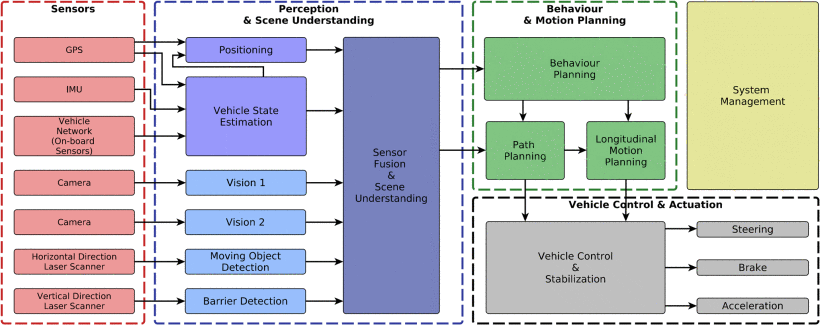
\includegraphics[width=\linewidth]{images/sota/ADS_information_flow.png}
    \label{sota_ads_information_flow}
    \caption{Arquitectura modular de un ADS. TEMPORAL!!!}
\end{figure}

En este tipo de arquitecturas, un error en una \mbox{sub-tarea} puede propagarse y afectar el desempeño de otras, comprometiendo así el funcionamiento del sistema. Esto es especialmente crítico en el módulo de percepción, ya que la calidad de la información obtenida impacta directamente en tareas posteriores como la localización, el mapeo y la planificación. Por ello, garantizar sistemas de percepción robustos es fundamental para el rendimiento y la seguridad de los \aclink{ADS}.

Dos de las tareas principales de los sistemas de percepción en los \aclink{ADS} son la detección 3D de objetos y la segmentación en \aclink{BEV}. La detección 3D de objetos es una de las tareas más relevantes y comúnmente se basa en nubes de puntos obtenidas mediante sensores LiDAR. En ausencia de LiDAR, una alternativa es la detección 3D multi-cámara, que busca predecir cajas delimitadoras 3D en un sistema de coordenadas \aclink{BEV} utilizando únicamente imágenes monoculares. Por otro lado, la segmentación en \aclink{BEV} tiene como objetivo realizar una segmentación semántica del entorno, identificando áreas transitables y delimitaciones de carril en el marco de referencia del vehículo. A diferencia de la detección de objetos, la segmentación en \aclink{BEV} permite una predicción densa de clases estáticas del entorno, lo que resulta clave para la construcción de mapas locales, estimación del comportamiento de agentes y downstream tasks como la planificación del comportamiento del \aclink{ADS}. \hl{Añadir referencias.}

% Parrafo conector que no se me ocurre nada
Este \aclink{TFM} se desarrolla en el contexto de la segmentación semántica en \aclink{BEV}\dots \hl{COMPLETAR.}


\subsection{Semantic segmentation}
\lipsum[2-4] % TODO

\subsection{BEV semantic segmentation}

% TODO: Esto es una piedra de ChatGPT y hay varios errores. Reescribir todo.
%       Alguna imagen no estaría de más.
%

Traditional methods (3D\_Traffic\_Scene\_Understanding) estimate local BEV maps using multi-camera input under the flat-ground assumption, applying Inverse Perspective Mapping (IPM). However, these methods require accurate camera parameters, which has led to research focusing on camera parameter estimation for BEV transformation (BEV\_Params\_Estimation1, BEV\_Params\_Estimation2).

Cam2BEV applies IPM to transform multi-camera input images into BEV space and refines the representation using homographies fed into the model. To handle occlusions, Cam2BEV introduces an additional semantic class that explicitly marks occluded areas from all vehicle-mounted cameras, improving the final BEV estimation.

HDMapNet generates high-definition semantic maps from multi-camera input by employing a feature projection module that transforms image features into BEV space. It models the 3D environment implicitly using an MLP and explicitly incorporates camera extrinsic parameters to project image-space features correctly into BEV. The model first extracts image features with a shared MLP backbone, transforms them into the camera coordinate system, and then projects them into BEV using camera extrinsics.

PYVA introduces a cross-view transformer that projects features from the front-view domain to the BEV domain. While similar to HDMapNet, PYVA differs in that it does not rely on camera parameters in the second transformation stage. Instead, it employs a GAN-based framework to manage occlusions, making it applicable for monocular settings but less suitable for multi-camera fusion.

Other approaches propose different architectures for BEV semantic segmentation. VPN introduces a two-layer MLP for multi-camera feature fusion, followed by a decoder for semantic segmentation in indoor environments. LSS presents a unified framework that lifts 2D images into 3D space by learning an implicit depth distribution, making it effective for end-to-end motion planning. M²BEV transforms 2D image features into 3D voxels along projection rays to generate an efficient BEV representation that supports tasks such as semantic segmentation and 3D object detection. BEVFormer, on the other hand, employs a transformer-based approach that aggregates spatial-temporal features from multi-view cameras and historical BEV frames, enhancing occlusion reasoning.

MonoLayout tackles occlusion estimation by employing a standard encoder-decoder framework combined with adversarial training, enabling it to predict amodal layouts of the driving scene. BEVFormer similarly enhances occlusion reasoning by leveraging attention mechanisms to fuse multi-view spatial-temporal features from historical BEV maps.

Several methods integrate multiple sensor modalities to improve BEV representations. FishingNet extends VPN by incorporating data from additional sensors, while HDMapNet also supports LiDAR fusion, allowing for a more detailed understanding of the driving environment.

To the best of our knowledge, Cam2BEV is the closest approach to this thesis. However, our work differs in several key aspects. Instead of applying semantic segmentation after transforming images into BEV space, we study whether training a segmentation model directly on BEV images improves the representation of planar elements compared to the traditional segmentation-first-then-IPM approach. Furthermore, we treat occupancy and occlusion mask generation as a post-processing step applied to BEV semantic segmentation. This is integrated into a pre-annotation pipeline for vehicle scenes, contributing to advancements in monocular 3D object detection.



\section{Metodology}
\label{metodologia}

% En esta sección se detallan los experimentos realizados para abordar las cuestiones propuestas en la sección \ref{Introduction}. En primer lugar, se introducen los detalles del diseño de la experimentación: la selección del modelo de segmentación, dataset elegido, procesos de entrenamiento y validación, etc. Después, se detalla el pipeline implementado para realizar la anotación semiautomática de las máscaras de ocupación, oclusión y área conducible. Finalmente, se aborda la metodología seguida para evaluar tanto la generación de las máscaras semánticas en \aclink{BEV}, como las detecciones 3D a partir de imágenes monoculares para la evaluación final del pipeline de anotación semiautomática.

This section details the experiments and implementations made to address the problems described in section \ref{Introduction}. On the first hand, the experimental design is introduced, tackling the model and dataset selection, how data augmentations are performed and the training and validation processes. Afterward, the implementation of the occupancy and occlusion masks preannotation pipeline is presented. Finally, the evaluation strategy of the pipeline is discussed to measure the quality of the resulting semantic masks and the monocular 3D detections for estimating the object's dimensions.

% Este proyecto puede dividirse en 3 bloques principales: experimentación con la segmentación semántica en BEV, diseño e implementación de un sistema de anotación semiautomático de máscaras de área conducible y un tercer bloque de experimentación para evaluar el rendimiento del sistema implementado.

Thus, this project can be divided into three main blocks: \aclink{BEV} semantic segmentation experimentation, design and implementation of the preannotation pipeline and a thrid block of how the system is evaluated.

\subsection{Segmentation experiment design: BEV2Seg\_2}
\label{bev2seg_2}

To address the hypotesis that "A semantic segmentation model trained with BEV images better segments planar elements" the process represented in Figure \ref{fig:beg2seg_2_flow} has been designed. It follows two main approaches: first, performing image segmentation on regular RGB images and then reprojecting them to \aclink{BEV}; second, applying \aclink{IPM} to the original images and then segmenting them with the model.

\begin{figure}[h!]
    \centering
    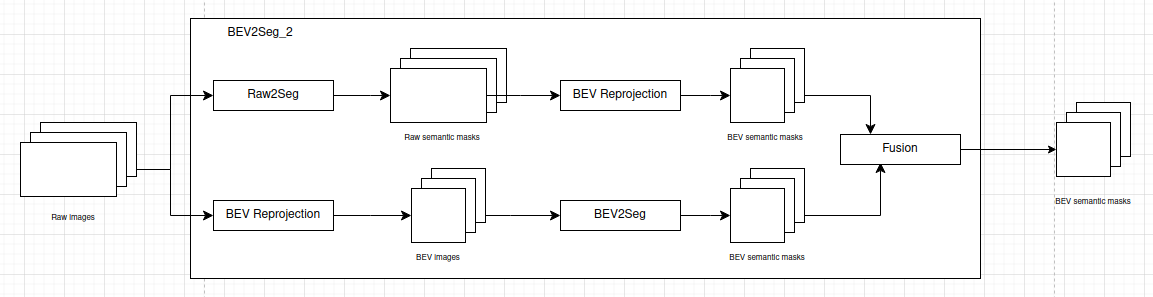
\includegraphics[width=\linewidth]{./images/metodology/bev2seg_2_flow.png}
    \caption{bev2seg\_2 diagram flow.}
    \label{fig:beg2seg_2_flow}
\end{figure}

Considering this flowchart, three main questions arises: (1) which segmentation model to use, (2) which dataset to train the models with, and (3) how to compare the train models and select the optimal output of the pipeline. 

\subsubsection{Segformer}
There are multiple techniques and strategies for tackling semantic segmentation in both regular and \aclink{BEV} images \ref{sota}.  

Several models could be chosen to address the proposed hypothesis. The current state of the art includes both \aclink{CNN} and \aclink{ViT}-based models that achieve competitive results. As shown in Figure \ref{tab:model_comparison}, there is no significant difference in accuracy and inference speed among the top-performing models. Moreover, many of these models have already been applied in the context of \aclink{ADS}. In this work, Segformer \cite{segformer} has been selected as the semantic segmentation model due to its balance between performance and efficiency. Additionally, it is integrated into the Huggingface \cite{huggingface} ecosystem, which provides an optimized, parallelized implementation, facilitating distributed training.  

\begin{table}[h]
    \centering
    \resizebox{\linewidth}{!}{%
    \begin{tabular}{l l c c c}
        \toprule
        \textbf{Model Name} & \textbf{Encoder} & \textbf{Params (M)} $\downarrow$ & \textbf{FPS} $\uparrow$ & \textbf{Cityscapes test mIoU ($\%$)} $\uparrow$ \\
        \midrule
        DDRNet-39       & -             & 32.3      & -         & 80.4 \\
        PIDNet-L        & -             & 36.9      & -         & 80.6 \\      
        DeeplabV3+      & ResNet-101    & 62.7      & 1.2       & 80.9 \\
        SETR            & ViT-Large     & 318.3     & 0.5       & 82.2 \\
        Segformer       & MiT-B4        & 64.1      & 3.0       & 83.8 \\
        \bottomrule
    \end{tabular}%
    }
    \caption{Comparison of different models. Results are obtained from \cite{DDRNet} \cite{PIDNet} \cite{segformer}.  }
    \label{tab:model_comparison}
\end{table}


The Segformer model consists on an hierarchical Transformer  encoder, which extract coarse and fine features, and a lightweight \aclink{MLP} decoder to directly fuse these multiscale features and predict the segmentation mask (Figure \ref{fig:segformer_architecture}). Segformer comes with a series of Mix Transformer encoders (MiT) that share the same architecture but have different sizes: from MiT-B0 as the lightweigtest encoder for realtime inference, to MiT-B5 for best performance.

\begin{figure}[h!]
    \centering
    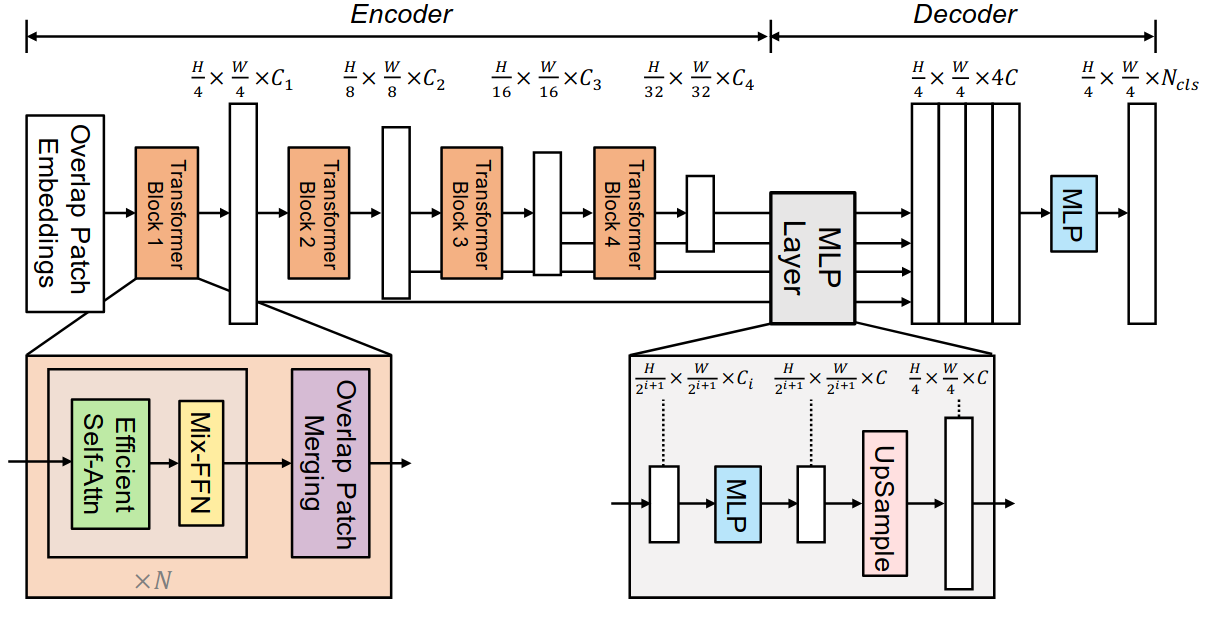
\includegraphics[width=\linewidth]{images/metodology/segformer_architecture.png}
    \caption{Segformer architecture}
    \label{fig:segformer_architecture}
\end{figure}

The training strategy involves using pretrained encoders from ImageNet-1K, attaching an untrained segmentation head decoder, and fine-tuning the entire model for semantic segmentation of vehicular scenes. Since the objective is to train the models directly on \aclink{BEV} images, which differ significantly from standard perspective images, the encoder layers will remain trainable rather than being frozen.


\subsubsection{BEVDataset}
In order to train the model on the segmentation task, a valid dataset must be selected. There are several semantic segmentation datasets for the \aclink{ADS} context such as Cityscapes \cite{Cityscapes}, that defines $30$ semantic classes and provides $5.000$ frames with pixel-level high-quality annotations and $20.000$ weakly annotated images; KITTI \cite{KITTI}, which provices $400$ annotated images with a $0.5$ split for training and validation following the Cityscapes annotation format; ApolloScape \cite{ApolloScape}, that provides $146.997$ frames with corresponding pixel-level annonations and pose information for $25$ labels; or NuImages, a subset of NuScenes \cite{nuscenes}, that contains annotated images on $26$ different labels. For all of them, the ego pose and camera parameters metadata are provided. 

There are other benchmarks \cite{WildDash} \cite{CamVid} but in orther to train the models a rich dataset is needed. Despite Cityscapes and ApolloScape being good options for this task, NuImages has been selected as it is one of the most used datasets for \aclink{ADS} tasks, it provides very accurate ego poses and camera parameters, it has 3D annotations and it has a very good documentation.

NuImages contains around $93.000$ samples with aproximately $80\%$ reserved for the training set and $20\%$ for validation. Additionally, NuImages includes a private test set reserved for benchmark evaluations, whose annotations are not publicly available.

To train the models in the pipeline, a parser has been developed to convert NuImages into a sub-dataset named BEVDataset. This dataset has all front-camera images with NuImages annotations. Since the test annotations in NuImages are private, the validation set has been further splitted to ensure fair comparisons between models from different pipelines.

The conversion process is performed using a custom parser named "OLDatasets", which transforms NuImages samples into the structured ASAM OpenLABEL \footnote{\url{https://www.asam.net/standards/detail/openlabel/}} format, where metadata for each frame is stored. In the case of BEVDataset, images are reprojected into the \aclink{BEV} domain using the \aclink{VCD} library. This library provides tools to handle OpenLABEL annotations and manage both 2D and 3D data efficiently.

The "OLDatasets" parser extracts the camera parameters for each sample and computes a \aclink{LUT} to apply \aclink{IPM} reprojection. Using this data, semantic pixel masks are generated and reprojected along with the original images into the \aclink{BEV} space. Since this reprojection involves image warping, the interpolation method must be carefully chosen:
\begin{itemize}
    \item Linear interpolation is applied to images.
    \item Nearest neighbor interpolation is used for semantic masks to preserve pixel class integrity. 
\end{itemize}

The virtual \aclink{BEV} camera parameters are fixed: the \aclink{BEV} reprojection is generated using a regular grid with a cell spacing of 1 meter, covering a total distance of 30 meters in front of the camera and 1 meter behind it. The resulting images have a resolution of $1024 \times 1024$ pixels.

Finally, BEVDataset contains a total of $16.427$ images, distributed as shown in Figure \ref{fig:bev_dataset}.

\begin{figure}[h!]
    \centering
    \includegraphics[width=\linewidth]{images/metodology/BEVDataset.png}
    \caption{BEVDataset structure and mini set samples}
    \label{fig:bev_dataset}
\end{figure}


\subsubsection{Data augmentations}
Data augmentations in \aclink{BEV} are not an easy task...

\subsubsection{Validation and comparison}
Mean intersection over union (mIoU) or Jaccard index is used as the metric for evaluation and comparison between the two approaches.

\subsection{ Driveable area automatic annotation}
\label{aplication}

\subsubsection{Depth estimation}
\subsubsection{Scene PCD}
\subsubsection{Instance scene PCD}
\subsubsection{Instance BEV mask}

\subsection{Evaluation methodology}
\label{evaluacion}

\subsubsection{3D detections evaluations}
\subsubsection{BEV masks evaluation}
\hl{Groundtruth BEV masks could be generated from annotations}




% \newpage
% \section*{acknowledgements}
% \label{acknowledgements}
% % ==========================================================
% =                   ACKNOWLEDGEMENTS                     =
% ==========================================================

Lore ipsum...
% 
% \newpage
% \section{Annexes}
% % ==========================================================
% =                         ANEXOS                         =
% ==========================================================
\phantomsection
\subsection*{OLDatasets}

Standing for OpenLABEL Datasets, OLDatasets is a custom parser from NuImages format to OpenLABEL format developed in order to integrate it with the \aclink{VCD} library ecosystem developed and maintained by Vicomtech \footnote{\url{https://www.vicomtech.org/en/}}.

\begin{table}[h]
    \centering
    \begin{tabular}{l c c c c}
        \toprule
        \textbf{Name} & \textbf{ID} & \textbf{trainId} & \textbf{Dynamic} & \textbf{Color (RGB)} \\
        \midrule
        background                          & 0  & 0  & False & (0, 0, 0) \\
        animal                              & 1  & 1  & True  & (255, 0, 0) \\
        human.pedestrian.adult              & 2  & 2  & True  & (220, 20, 60) \\
        human.pedestrian.child              & 3  & 3  & True  & (220, 20, 60) \\
        human.pedestrian.construction\_worker & 4  & 4  & True  & (220, 20, 60) \\
        human.pedestrian.personal\_mobility & 5  & 5  & True  & (220, 20, 60) \\
        human.pedestrian.police\_officer    & 6  & 6  & True  & (220, 20, 60) \\
        human.pedestrian.stroller           & 7  & 7  & True  & (220, 20, 60) \\
        human.pedestrian.wheelchair         & 8  & 8  & True  & (220, 20, 60) \\
        movable\_object.barrier             & 9  & 9  & False & (190, 153, 153) \\
        movable\_object.debris              & 10 & 10 & False & (152, 251, 152) \\
        movable\_object.pushable\_pullable  & 11 & 11 & False & (255, 0, 0) \\
        movable\_object.trafficcone         & 12 & 12 & True  & (111, 74, 0) \\
        static\_object.bicycle\_rack        & 13 & 13 & False & (255, 0, 0) \\
        vehicle.bicycle                     & 14 & 14 & True  & (119, 11, 32) \\
        vehicle.bus.bendy                   & 15 & 15 & True  & (0, 60, 100) \\
        vehicle.bus.rigid                   & 16 & 16 & True  & (0, 60, 100) \\
        vehicle.car                         & 17 & 17 & True  & (0, 0, 142) \\
        vehicle.construction                & 18 & 18 & True  & (255, 0, 0) \\
        vehicle.emergency.ambulance         & 19 & 19 & True  & (255, 0, 0) \\
        vehicle.emergency.police            & 20 & 20 & True  & (255, 0, 0) \\
        vehicle.motorcycle                  & 21 & 21 & True  & (0, 0, 230) \\
        vehicle.trailer                     & 22 & 22 & True  & (0, 0, 110) \\
        vehicle.truck                       & 23 & 23 & True  & (0, 0, 70) \\
        vehicle.ego                         & 24 & 24 & True  & (255, 255, 255) \\
        flat.driveable\_surface             & 25 & 25 & False & (128, 64, 128) \\
        \midrule
        ignore                              & 255 & 255 &       &        \\
        \bottomrule
    \end{tabular}
    \caption{Semantic labels defined for NuImages masks}
    \label{tab:semantic_labels}
\end{table}

\begin{figure}[h!]
    \centering
    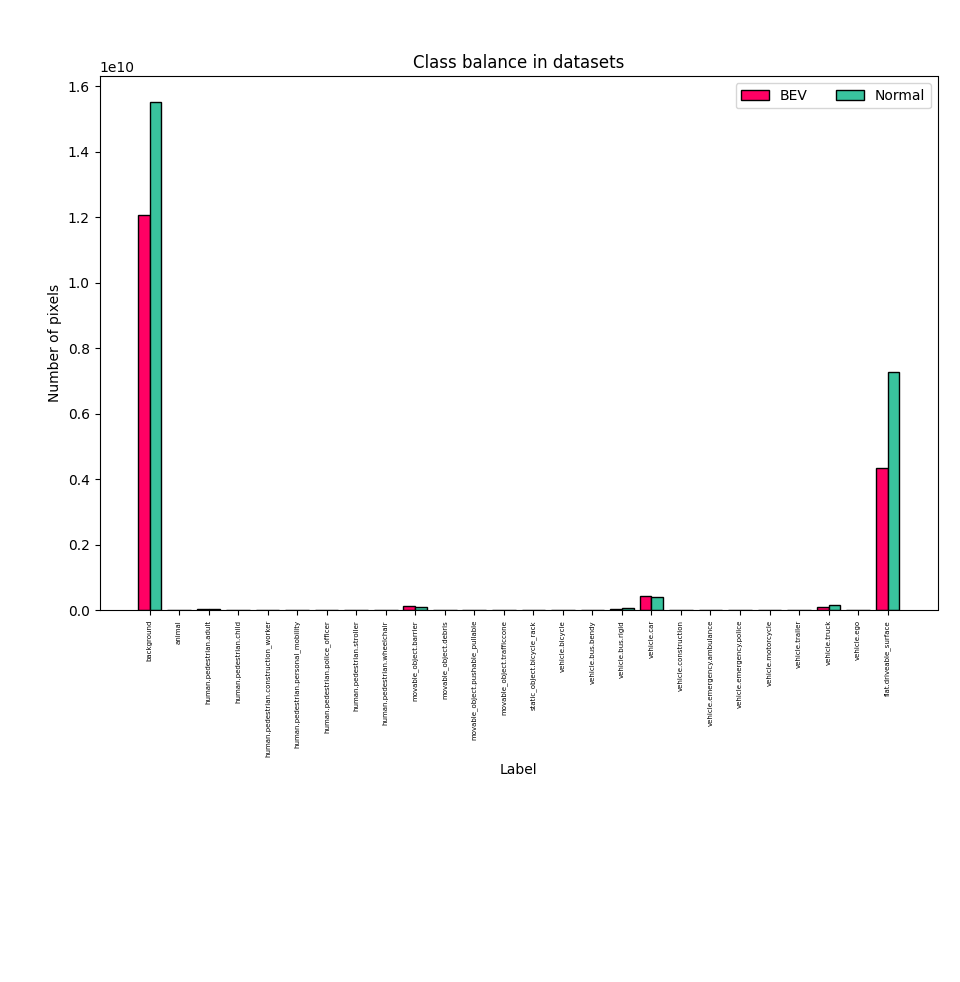
\includegraphics[width=\linewidth]{images/methodology/dataset_class_balance.png}
    \caption{Dataset class balance}
    \label{fig:dataset_class_balance}
\end{figure}

\subsection*{Rotation matrix to euler angles}
Here \cite{euler_from_matrix} is the pseudocode.


\subsection*{Color palette}
\begin{table}[h]
    \centering
    \renewcommand{\arraystretch}{1.5} % Increase row height
    \setlength{\tabcolsep}{12pt} % Increase column spacing
    \begin{tabular}{c c}
        \toprule
        \textbf{Hex Code} & \textbf{Color Sample} \\
        \midrule
        \#F44336 & \cellcolor[HTML]{F44336} \hspace{2cm} \\
        \#EF5350 & \cellcolor[HTML]{EF5350} \hspace{2cm} \\
        \#F1464E & \cellcolor[HTML]{F1464E} \hspace{2cm} \\
        \#FF9800 & \cellcolor[HTML]{FF9800} \hspace{2cm} \\
        \#FF0064 & \cellcolor[HTML]{FF0064} \hspace{2cm} \\
        \midrule
        \#4CAF50 & \cellcolor[HTML]{4CAF50} \hspace{2cm} \\
        \#86BB48 & \cellcolor[HTML]{86BB48} \hspace{2cm} \\
        \#39C39E & \cellcolor[HTML]{39C39E} \hspace{2cm} \\
        \midrule
        \#0277BD & \cellcolor[HTML]{0277BD} \hspace{2cm} \\
        \#0097A7 & \cellcolor[HTML]{0097A7} \hspace{2cm} \\
        \#2AB0D2 & \cellcolor[HTML]{2AB0D2} \hspace{2cm} \\
        \#01A1FF & \cellcolor[HTML]{01A1FF} \hspace{2cm} \\
        \#0073B7 & \cellcolor[HTML]{0073B7} \hspace{2cm} \\
        \bottomrule
    \end{tabular}
    \caption{Color Palette}
    \label{tab:color_palette}
\end{table}


\newpage\printbibliography
\addcontentsline{toc}{section}{References}

\end{document}
